\section*{Unbounded arrays%
\TAGS{array, ds-invariant}}

When implementing unbounded arrays on an embedded device, a programmer
is concerned that doubling the size of the array when we reach its
limit may use precious memory resources too aggressively.  So she
decides to see if she can increase it by a factor of $\frac{3}{2} =
1.5$ instead, rounding down if the result is not an integral number.
\begin{center}
  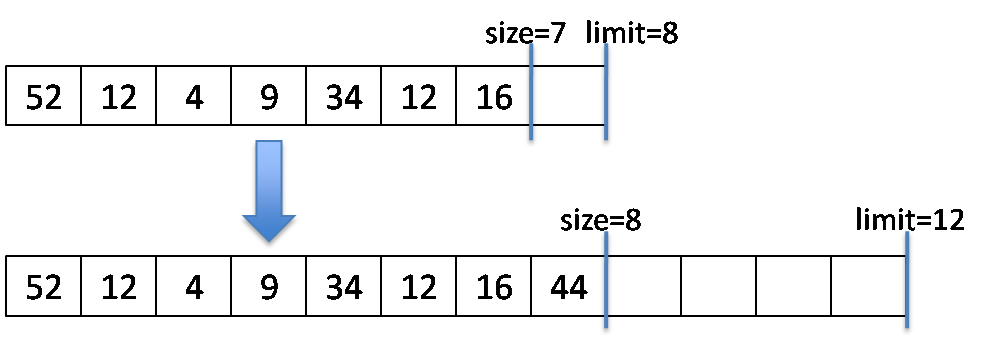
\includegraphics[width=0.6\textwidth]{\img/uba.png}
\end{center}
This means that it won't make sense for the limit to be less than
\shortanswerline{\hspace{1em}2\hspace{1em}}, because otherwise you
might resize the array and get an array that wasn't any bigger. This
needs to be reflected in the data structure invariant!

\begin{lstlisting}[numbers=left, name="uba_header", belowskip=0pt]
struct uba_header {
  int size;
  int limit;
  string[] data;
};
typedef struct uba_header uba;

bool is_arr_expected_length(string[] A, int limit) {
  //@assert \length(A) == limit;
  return true;
}

bool is_uba(uba* A) {
\end{lstlisting}
\begin{lstlisting}[numbers=left, name="uba_header", aboveskip=0pt, belowskip=0pt, lineskip=2ex]
    [*\answerline{return A != NULL \&\& 2 <= A->limit}*]
    [*\answerline{\hspace{1em}\&\& is\_arr\_expected\_length(A->data, A->limit)}*]
    [*\answerline{\hspace{1em}\&\& 0 <= A->size \&\& A->size < A->limit;}*]
  \end{lstlisting}
\begin{lstlisting}[numbers=left, name="uba_header", aboveskip=0pt]
}

\end{lstlisting}